% This file allows to produce either a separate PDF/PNG image
% See standalone documentation to understand underlying magic

\documentclass[tikz,convert={density=150,size=600,outext=.png}]{standalone}
\usetikzlibrary{shapes, calc, arrows, fit, positioning, decorations, patterns, decorations.pathreplacing, chains, snakes}
\input{../setup-web-fonts}
\input{../setup-packages}
\graphicspath{{../pictures/}} % path to pictures, trailing slash is mandatory.

\begin{document}

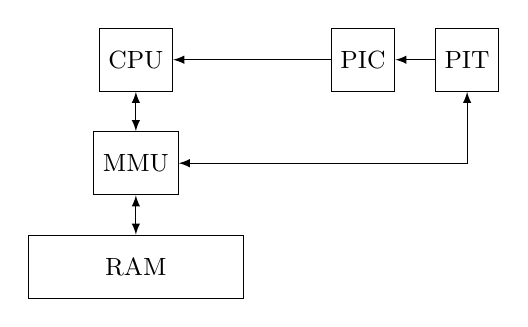
\begin{tikzpicture}[>=latex, font=\small, node distance = 0.5cm]

\begin{scope}[minimum height=0.8cm]
    \node[draw, ] (cpu) {CPU};
    \node[draw, below=of cpu] (mmu) {MMU};
    \node[draw, right=2cm of cpu, ] (pic) {PIC};

    \node[draw, below=of mmu, text width=2.5cm, align = center, ] (dram) {RAM};
    \node[draw, right=of pic, ] (pit) {PIT};

\end{scope}

\draw[<->] (cpu) -- (mmu); // node[midway] {/};
\draw[<->] (mmu) -- (dram);

\draw[<->] (mmu) -| (pit);

\draw[->, ] (pic) -- (cpu);
\draw[->, ] (pit) -- (pic);

\end{tikzpicture}

\end{document}
